\chapter{関連研究・関連技術}
\label{chap:related_works}

本章では,本研究の提案手法を述べる前に関連研究や関連技術,その問題点について記述する.

\section{Intel VT: Virtualization Technology}
\label{sec:vt}

Intelは2005年にx86アーキテクチャ上での仮想マシンの実行をサポートし,仮想化オーバーヘッドを
削減するための技術である
VTを発表した\cite{intelsdm}.VTはハードウェアレベルで仮想マシンの実行をサポートするいくつかの
コンポーネントからなり,そのうちの1つにVT-xがある.

VT-xはCPUやメモリの仮想化を支援する機構であり,後述するVMCSや
EPTはVT-xの機能である.
VT-xでは仮想化を支援するためにプロセッサにVMX root,VMX non-rootの2つの動作モードが
設定された.
VMX rootモードはVMMが動作するモードであり,VMX non-rootモードはゲストOSが動作するモードである.
ゲストOSがハードウェアリソースへのアクセスなどのセンシティブ命令を実行した場合,VMEXITと
呼ばれるVMX rootモードへの遷移が発生し,VMMが必要な処理を行うことが出来る.
VMX non-rootモードへの遷移はVMENTRYと呼ばれる.

\section{VMCS: Virtual-Machine Control Structure}
\label{sec:vmcs}

CPUはVMCSと呼ばれる構造体を用いてVMX root,VMX non-rootモードそれぞれへの遷移や
VMX non-rootモードでの動作時の挙動を管理している\cite{intelsdm}.
VMCSはホストのメモリ上に確保され,VMPTRLD命令によってCPUに登録される.
VMWREAD,VMWRITEといったVMX命令を用いてVMCSの各フィールドの値を読み書きすることができる.

\section{EPT: Extended Page Table}
\label{sec:ept}

Intel CPUはNehalemアーキテクチャ以降,ゲスト物理アドレス(GPA)からホスト物理アドレス(HPA)への
アドレス変換をハードウェアで支援するEPTを採用している\cite{nehalem}.
vCPUが物理メモリ上のデータにアクセスする場合
GPAを利用してメモリアクセスを行おうとする.EPTを利用する環境においては,CPUがEPTを参照し,
GPAをHPAに置き換えてメモリアクセスを実施する.
これによりシャドウページテーブルを用いた既存手法と比較して,GPAからHPAへのアドレス変換が大幅に高速化された.
VMWRITE命令を用いてVMCSにEPTのポインタを登録することで,CPUはEPTのメモリ上での位置を知り,利用することが出来る.

\section{ネスト仮想化}
\label{sec:nested_virtualization}

ネスト仮想化はPopek, Goldberg\cite{popek_goldberg}によって提唱された,
仮想マシン上で仮想マシンを実行するという概念である.
しかし,x86アーキテクチャではネスト仮想化がサポートされないため,どれだけネストされた
仮想マシンであっても1つのVMMがトラップをハンドリングすることになる.
そのため,ネスト仮想化に関する処理はVMM中に実装される必要がある.
KVMにおけるネスト仮想化はBen-Yehudaらによって実装された\cite{turtles}.

(まだ詳細を書き足す)
(Nested-VMのvCPUに対応するVMCSがベアメタルマシン上で動作するホストOS上に存在することを記述する
必要がある)

\section{既存手法}
\label{subsec:existing_method}

VMにメモリフォレンジックを行うためにはVMのメモリ空間を復元しなければならない.
これを実現するためにはVMやそのvCPUの数,EPTのアドレス,ネスト仮想化の有無
といった情報を把握する必要がある.Intel VT環境においてはこのような情報は
VMCSから得ることができる.

しかし,VMCS内の各フィールドのメモリ上でのオフセットはアーキテクチャによって異なる上,
公開されていない.
フィールドへの読み書きはVMREAD,VMWRITE命令を通じて行われるため
VMMがこれを意識することはないが,
この仕様はシグネチャマッチングなどを用いたVMCSのメモリ中からの発見を
困難にしている.

Grazianoら\cite{hypervisor_memory_forensics}はVMCS領域に
値をインクリメントした2バイト単位のデータ列を配置した後,
VMREAD命令を用いて各フィールドの値を読み出すことで
VMCSのメモリレイアウトを復元することに成功した.これによりVMCSをメモリ中から
探索することが可能になった.復元されたVMCSに格納されている
物理CPU,vCPUのCR3レジスタの値を比較することでVMの構成を復元,
EPTPフィールドを読み出すことでvCPUが使用するEPTのアドレスを取得し,
VMにメモリフォレンジックを行うことが可能になった.
Zhangら\cite{kvm_vm_forensics}はこの手法を用いてKVM上の仮想マシンの
詳細な情報を取得することに成功した.

\section{既存手法の問題}
\label{subsec:problem_with_existing_method}

IntelプロセッサはCPUの内部にVMCSを格納するための
記憶領域を保持している.そのため,VMWRITE命令を用いて
VMCSSのフィールドに値を書き込んだとしても,メモリ上のVMCS領域に値が反映される
保証はない\cite{intelsdm}\cite{rekall}(図\ref{fig:problem}).Grazianoらが提案した手法
\cite{hypervisor_memory_forensics}やそれを利用した後続の研究\cite{kvm_vm_forensics}では
VMCSをシグネチャマッチングでメモリ上から探索しているため,
このような機構が存在するXeon WestmereやHaswell以降の
比較的モダンなIntelプロセッサには適用できないという問題がある.

\begin{figure}[h]
  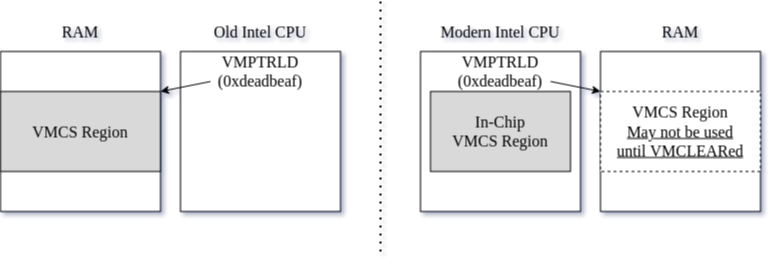
\includegraphics[scale=0.305]{problem.png}
  \caption{CPU内に存在するVMCS記憶領域}
  \label{fig:problem}
\end{figure}
